\chapter{Kerr 振子：非线性与量子回复}
\label{ch:kerr}

\begin{learningobjectives}
完成本章后，读者应能：
\begin{enumerate}
  \item 求解相干态在 Kerr 哈密顿量下的一阶相干性；
  \item 从四次算符的 Weyl 符号推导 TWA 漂移；
  \item 区分相位剪切造成的塌缩和离散能谱造成的量子回复；
  \item 用精确解量化 TWA 的早期准确性与长时间失效。
\end{enumerate}
\end{learningobjectives}

\section{最小的非线性多体模型}

单模 Kerr 哈密顿量为
\begin{equation}
  \Hhat=\frac{\hbar\chi}{2}\had\had\ha\ha
  =\frac{\hbar\chi}{2}\hat n(\hat n-1).
  \label{eq:kerr-hamiltonian}
\end{equation}
它保持粒子数，却使不同 Fock 分量积累不同相位。尽管只有一个模式，这个模型已经同时包含 TWA 最擅长和最难处理的现象：初期的相空间相位剪切可由经典轨迹描述，长时间的量子回复则依赖离散谱的相位重新对齐。
把这一可解模型作为半经典动力学和 TWA 的短时基准，也与相空间展开的
通用分析框架一致\cite{Polkovnikov2003,Polkovnikov2010}。

设初态为相干态 $\ket{\alpha_0}$，平均占据 $N=|\alpha_0|^2$。Fock 展开为
\begin{equation}
  \ket{\alpha_0}=\ee^{-N/2}
  \sum_{n=0}^{\infty}\frac{\alpha_0^n}{\sqrt{n!}}\ket n.
\end{equation}
能级为 $E_n=\hbar\chi n(n-1)/2$。相邻能级差 $E_n-E_{n-1}=\hbar\chi(n-1)$ 决定 $\qavg{\ha(t)}$ 的相位，直接求和得到
\begin{equation}
  \qavg{\ha(t)}_{\mathrm{exact}}
  =\alpha_0\exp\!\left[N(\ee^{-\ii\chi t}-1)\right].
  \label{eq:kerr-exact-mean}
\end{equation}

相干性的模为
\begin{equation}
  \frac{|\qavg{\ha(t)}|}{|\alpha_0|}
  =\exp[N(\cos\chi t-1)].
  \label{eq:kerr-exact-coherence}
\end{equation}
在 $|\chi t|\ll1$ 时，\cref{eq:kerr-exact-coherence} 近似为 $\exp[-N(\chi t)^2/2]$，塌缩时间尺度约为 $(\chi\sqrt N)^{-1}$。在 $\chi t=2\pi$ 时，所有离散 Fock 分量重新对齐，出现完整回复。

\section{Kerr 哈密顿量的 Weyl 符号}

利用第2章的四阶 Weyl 符号，
\begin{equation}
  H_W(\alpha,\alpha^*)
  =\frac{\hbar\chi}{2}
  \left(|\alpha|^4-2|\alpha|^2+\frac12\right).
  \label{eq:kerr-weyl-hamiltonian}
\end{equation}
截去精确 Wigner 方程中的三阶导数后，漂移方程为
\begin{equation}
  \ii\frac{\dd\alpha}{\dd t}
  =\frac{1}{\hbar}\pder{H_W}{\alpha^*}
  =\chi(|\alpha|^2-1)\alpha.
  \label{eq:kerr-twa-drift}
\end{equation}
每条轨迹的 $|\alpha|^2$ 守恒，所以解析解为
\begin{equation}
  \alpha(t)=\alpha(0)
  \exp[-\ii\chi(|\alpha(0)|^2-1)t].
  \label{eq:kerr-twa-trajectory}
\end{equation}
第7章将用 Bopp 算符把这里被省略的两个混合三阶导数完整展开，并给出其相对于领先漂移的 $1/N$ 计数。
相干态初值仍按
\begin{equation}
  \alpha(0)=\alpha_0+\frac{\xi_1+\ii\xi_2}{2}
\end{equation}
抽样。不同样本具有略微不同的半径，因而具有不同角速度；系综平均相干性随相位云团剪切而衰减。

\begin{intuitionbox}
早期塌缩不要求环境耗散。它可以只是不同粒子数分量或不同相空间半径的可逆去相位。量子回复则要求这些离散分量在特定时刻重新对齐；连续的经典轨迹频率分布通常不能重建这种干涉。
\end{intuitionbox}

\section{精确解与 TWA 的实际比较}

\cref{fig:kerr-exact-vs-twa} 使用 $N=9$，以 $\tau=\chi t$ 为无量纲时间。精确曲线由\cref{eq:kerr-exact-mean} 计算，TWA 曲线由 $100000$ 个真实随机初值和\cref{eq:kerr-twa-trajectory} 计算。

\begin{figure}[htbp]
  \centering
  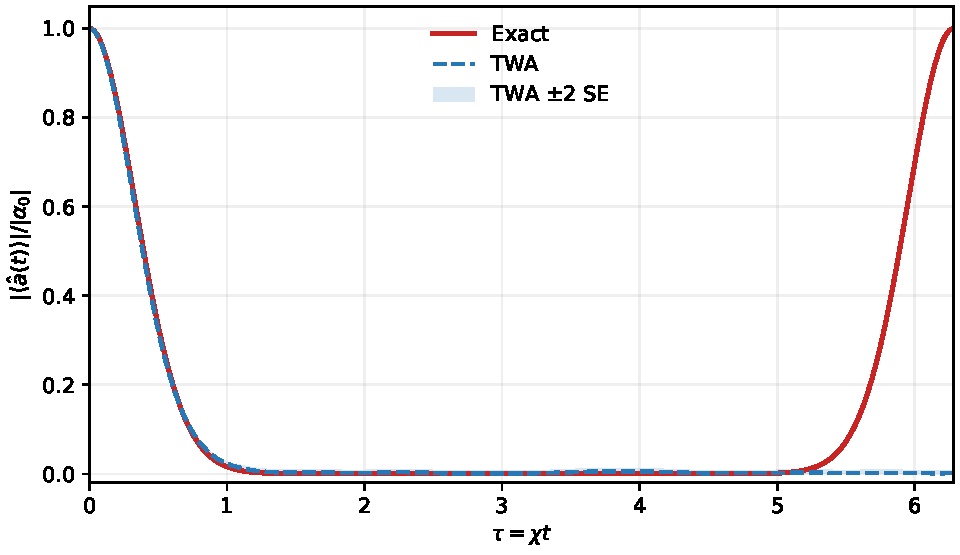
\includegraphics[width=0.82\textwidth]{figures/ch06/kerr_exact_vs_twa.pdf}
  \caption[Kerr 精确动力学与 TWA 的塌缩--回复对照]{相干态 Kerr 动力学的一阶相干性。黑线为 $N=9$ 的精确结果，蓝线为 $100000$ 条 TWA 轨迹的平均，阴影为 $\pm2$ 标准误。TWA 在所标早期窗口内再现塌缩，却不能在 $\tau=2\pi$ 重建量子回复；这张图检验的是该特定初态与观测量，不能据此宣称长时间 TWA 普遍有效。图由 \texttt{code/ch06\_kerr/kerr\_exact\_vs\_twa.py} 实际计算。}
  \label{fig:kerr-exact-vs-twa}
\end{figure}

在 $\tau\le0.25$ 的窗口内，归一化相干性最大绝对偏差为 $1.016\times10^{-2}$。在回复时刻，精确值为 $1$，TWA 为 $2.13\times10^{-3}$，其标准误为 $3.25\times10^{-3}$；即使计入 $4$ 个标准误，也与精确回复相差悬殊。正规排序粒子数的 TWA 初始估计为 $8.99958\pm0.00963$，解析值为 $9$；粒子数随后在每条 TWA 轨迹上保持。

这里的长时间差异不是轨迹数不足。继续增加轨迹数只会使 TWA 曲线更精确地趋近其连续经典系综极限，不会产生缺失的量子回复。完整指标保存在
\begin{center}
  \path{data/ch06/kerr_metrics.json}。
\end{center}

\section{塌缩不是热化}

Kerr 模型只有一个守恒占据和一个相位自由度，不具备在大量模式间重新分配能量的机制。$\qavg{\ha(t)}$ 的衰减是相位混合，不是热浴耗散，也不是多体碰撞热化。精确量子系统在 $2\pi/\chi$ 后回复，进一步证明早期衰减没有丢失信息。

在多模系统中，相位混合、动力学不稳定和真实的模式间散射可以同时发生。只观察一个相干因子下降，无法区分这些机制。需要结合模式占据、守恒量、可逆协议、关联函数和时间尺度判断。

\section{Weyl 修正为什么重要}

若错误地使用
\begin{equation}
  \ii\dot\alpha=\chi|\alpha|^2\alpha
\end{equation}
而忽略\cref{eq:kerr-twa-drift} 中的 $-1$，单条轨迹频率会整体偏移。对高占据 $N\gg1$，相对误差约为 $1/N$，短时间看似很小；但相位误差随时间积累，长时间比较会显著偏离。这个 $-1$ 来自哈密顿量的 Weyl 符号，不应通过经验调参补偿。

\begin{warningbox}
TWA 能准确描述塌缩，并不说明它也能描述随后的回复。判断有效性必须针对具体观测量和时间窗口，而不能只凭某个早期曲线吻合后把计算无限延长。
\end{warningbox}

\section{从 Kerr 模型学到的验证策略}

一个非线性 TWA 程序至少应通过以下检查：
\begin{enumerate}
  \item 在 $\chi=0$ 时退化为第5章的二次精确传播；
  \item 每条闭合轨迹保持 $|\alpha|^2$ 和 $H_W$；
  \item 相干态初始矩满足半量子修正；
  \item 在短时间窗口与\cref{eq:kerr-exact-mean} 收敛；
  \item 明确展示量子回复等已知失效现象，而不是隐藏长时间差异。
\end{enumerate}

\section*{本章小结}

Kerr 振子把 TWA 的能力边界压缩在一个可精确求解的模型中。非线性相位剪切造成的早期塌缩可以由初始 Wigner 涨落和经典漂移描述；离散量子谱造成的回复需要被截去的量子干涉。实际计算验证了早期吻合和长时间失效，并说明增加轨迹数不能修复方法误差。

\begin{exercises}
  \item 从 Fock 展开推导\cref{eq:kerr-exact-mean}。
  \item 由\cref{eq:kerr-weyl-hamiltonian} 推导\cref{eq:kerr-twa-drift}，解释频率中的 $-1$。
  \item 求精确相干性的半高宽随 $N$ 的标度。
  \item 修改程序比较 $N=1,9,100$，研究固定短时间窗口内的误差怎样随占据变化。
  \item 设计一次反转 $\chi\to-\chi$ 的回波协议，并比较精确动力学与数值积分误差。
\end{exercises}
